\documentclass[10pt,twoside,english,a4paper]{article}
%I can write this in English
% Engineering methods

\usepackage{graphicx} % Required for inserting images

%\usepackage[T1]{fontenc}
\usepackage[IL2]{fontenc} % lepšia sadzba písmena Ľ než v T1
\usepackage[utf8]{inputenc}
\usepackage{url} % príkaz \url na formátovanie URL
\usepackage{hyperref} % odkazy v texte budú aktívne (pri niektorých triedach dokumentov spôsobuje posun textu)
\usepackage{amsmath}
\usepackage{cite}
\graphicspath{{images/}}
%\usepackage{times}

\pagestyle{headings}

\title{Delivering Relevant Product Recommendations in Finance\thanks{Semester project from subject Engineering methods, academic year 2024/25, management: Martin Sabo}} % 

\author{Mykhailo Chepara\\[2pt]
	{\small Slovak Technical University in Bratislava}\\
	{\small Faculty of Information and Information Technologies}\\
	{\small \texttt{xchepara@stuba.sk}}
	}

\date{\small October 1 2024} % upravte



\begin{document}


\maketitle

\begin{abstract}
To begin with why is that topic? 
One of my friends is working in a financing company, therefore I'm genuinely curious how does a bank recommend products to it's customers. It's a useful tool for a bank to increase it's revenue but can it be enhanced? And if yes then how?

Now to the points that I'm going to untangle in this article:
\begin{itemize}
    \item What is a recommendation system
    \item Distribution of the systems based on thier architecture
    \item Usage cases in real life
    \item How does a recommendation system in a bank work
    \begin{itemize} 
             \item Architecture and ways of utilizing data
             \item Algorithms applied
             \item Data types used
    \end{itemize}
    
    \item Conditions to be met before deployment of the system
    \begin{itemize}
        \item Learning conditions
        \item Duration of learning
        \item And other conditions
    \end{itemize}
    
    \item Issues with the system
    \begin{itemize}
        \item Lack of data
        \item New item introduction
        \item Unability to recommend anything relevant to a user
        \item And other isssues
    \end{itemize}
    
    \item Enhancement of the system
    \begin{itemize}
        \item Possibility of merging a recommendation system with another system
        \item Systems that can be merged with recommendation system
        \item Resolving problems occuring in the system
        \item Other improvements
    \end{itemize}
    

\end{itemize}


\end{abstract}


\tableofcontents
\newpage










\section{Recommendation system}

\subsection{Definition of a recommendation system and its objective}
Nowadays people buy a lot of things on the internet, they watch a lot of films and do a lot of other stuff. Since there's such a rich amount of choises it's hard to find the ones people would choose. For that reason reommandation system was introduced. A recommendation system also called recommender system is a program which recommends user a product/service which he/she most probably would buy. The system is trained on huge amounts of data. Ultimately it tries to predict next probable choise of a customer and then recommends it. It could be next film watched, next purchase bought or next route on the road recommended. The data is provided by the customer's overall experience. It could be purchases, filmes watched, time used on app and so on. So it's a system adapting to each customer's needs and preferences.\cite{vars_rec_sys}

\subsection{Distribution of the systems based on thier architecture}
The systems are divided into few main categories. Some of them are content-based systems, collaborative systems and hybrid systems. Here is a graph of them in detail
\begin{figure}[h]
\centering
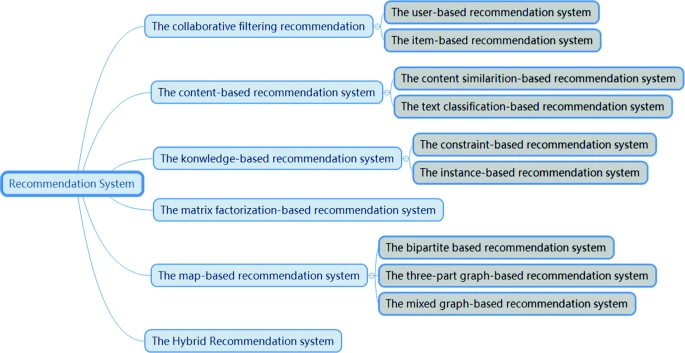
\includegraphics[width=0.8\textwidth]{system_vars}
\caption{Distribution of systems based on the architecture}\cite{wang2019review}
\label{fig:System categories}
\end{figure}
\par Collaborative filtering is one of the most used types of recommendation systems in the world. Collaborative filtering recommends something based on preferences of another user which has common traits with the current one. 

Advantages of the system type:
\begin{itemize}
\item Filtering complex information:
It can filter information which is hard to analyze automatically by machines, that is music, art etc. 
\item Recommending completely new information:
It's able to recommend utterly distingush information to the one introduced prior
\item Utilizing feedback of similar users:
It effectively use info of other similar users to the current one and give out useful results
\end{itemize}

Disadvantages of the system type
\begin{itemize}
\item Rarity:
Amount of projects and users is big and useres don't rate each and every project used therefore there are no common scores between them, resulting in similarity cannot be calculated
\item Multiple Content:
Colaborative filtering doesn't take into account influence of categories onto the recommendation
\item Scalability:
The number of users and projects is increasing each day. Henceforth system needs more and more time to compute bigger and bigger matrices of users and projects. So the probem of scalability occurs.
\end{itemize}

\par Content-based filtering is the most used type of systems in academic search engines. The plain idea of it is to record which object user has chosen from list of recommended objects and then analyze it, based on that it recommends next the most relevant object. For example it can recommend an article with attributes academic, fresh and popular. The point is to recommend an object which has biggest similarity by description to the description provided by user.
Content-based recommendations consists of the following three steps:
\begin{itemize}
\item Extracting features and build model that descibe resources
\item Compare current features's similarity with previous features's in order to decide if recommendation is viable
\item In conformance to similarity of the items to current item an array of items is selected and recommended to user
\end{itemize}
Advantages
\begin{itemize}
\item It doesn't need data of other users, and can start working without it
\item It's able to adapt to user's individual preferences in order to make personalized recommendations
\item It can recommend any new projects, no problem with new objects recommendations
\item It can be easily explained why objects are recommended based on their characteristics and current preferenced characteristics
\end{itemize}

Disadvantages
\begin{itemize}
\item If user changes his profile his preferences are gone, and now system needs to adapt to user's preferences again
\item There's a possibility that system will recommend the same product user liked before
\item Problem of lack of the history, thus at the beginning there's no data provided by user which mean the accuracy is low
\end{itemize}

\subsection{Usage cases in real life}
Here are the main variations of recommendation systems which are used the most commonly.

\begin{figure}[h]
\centering
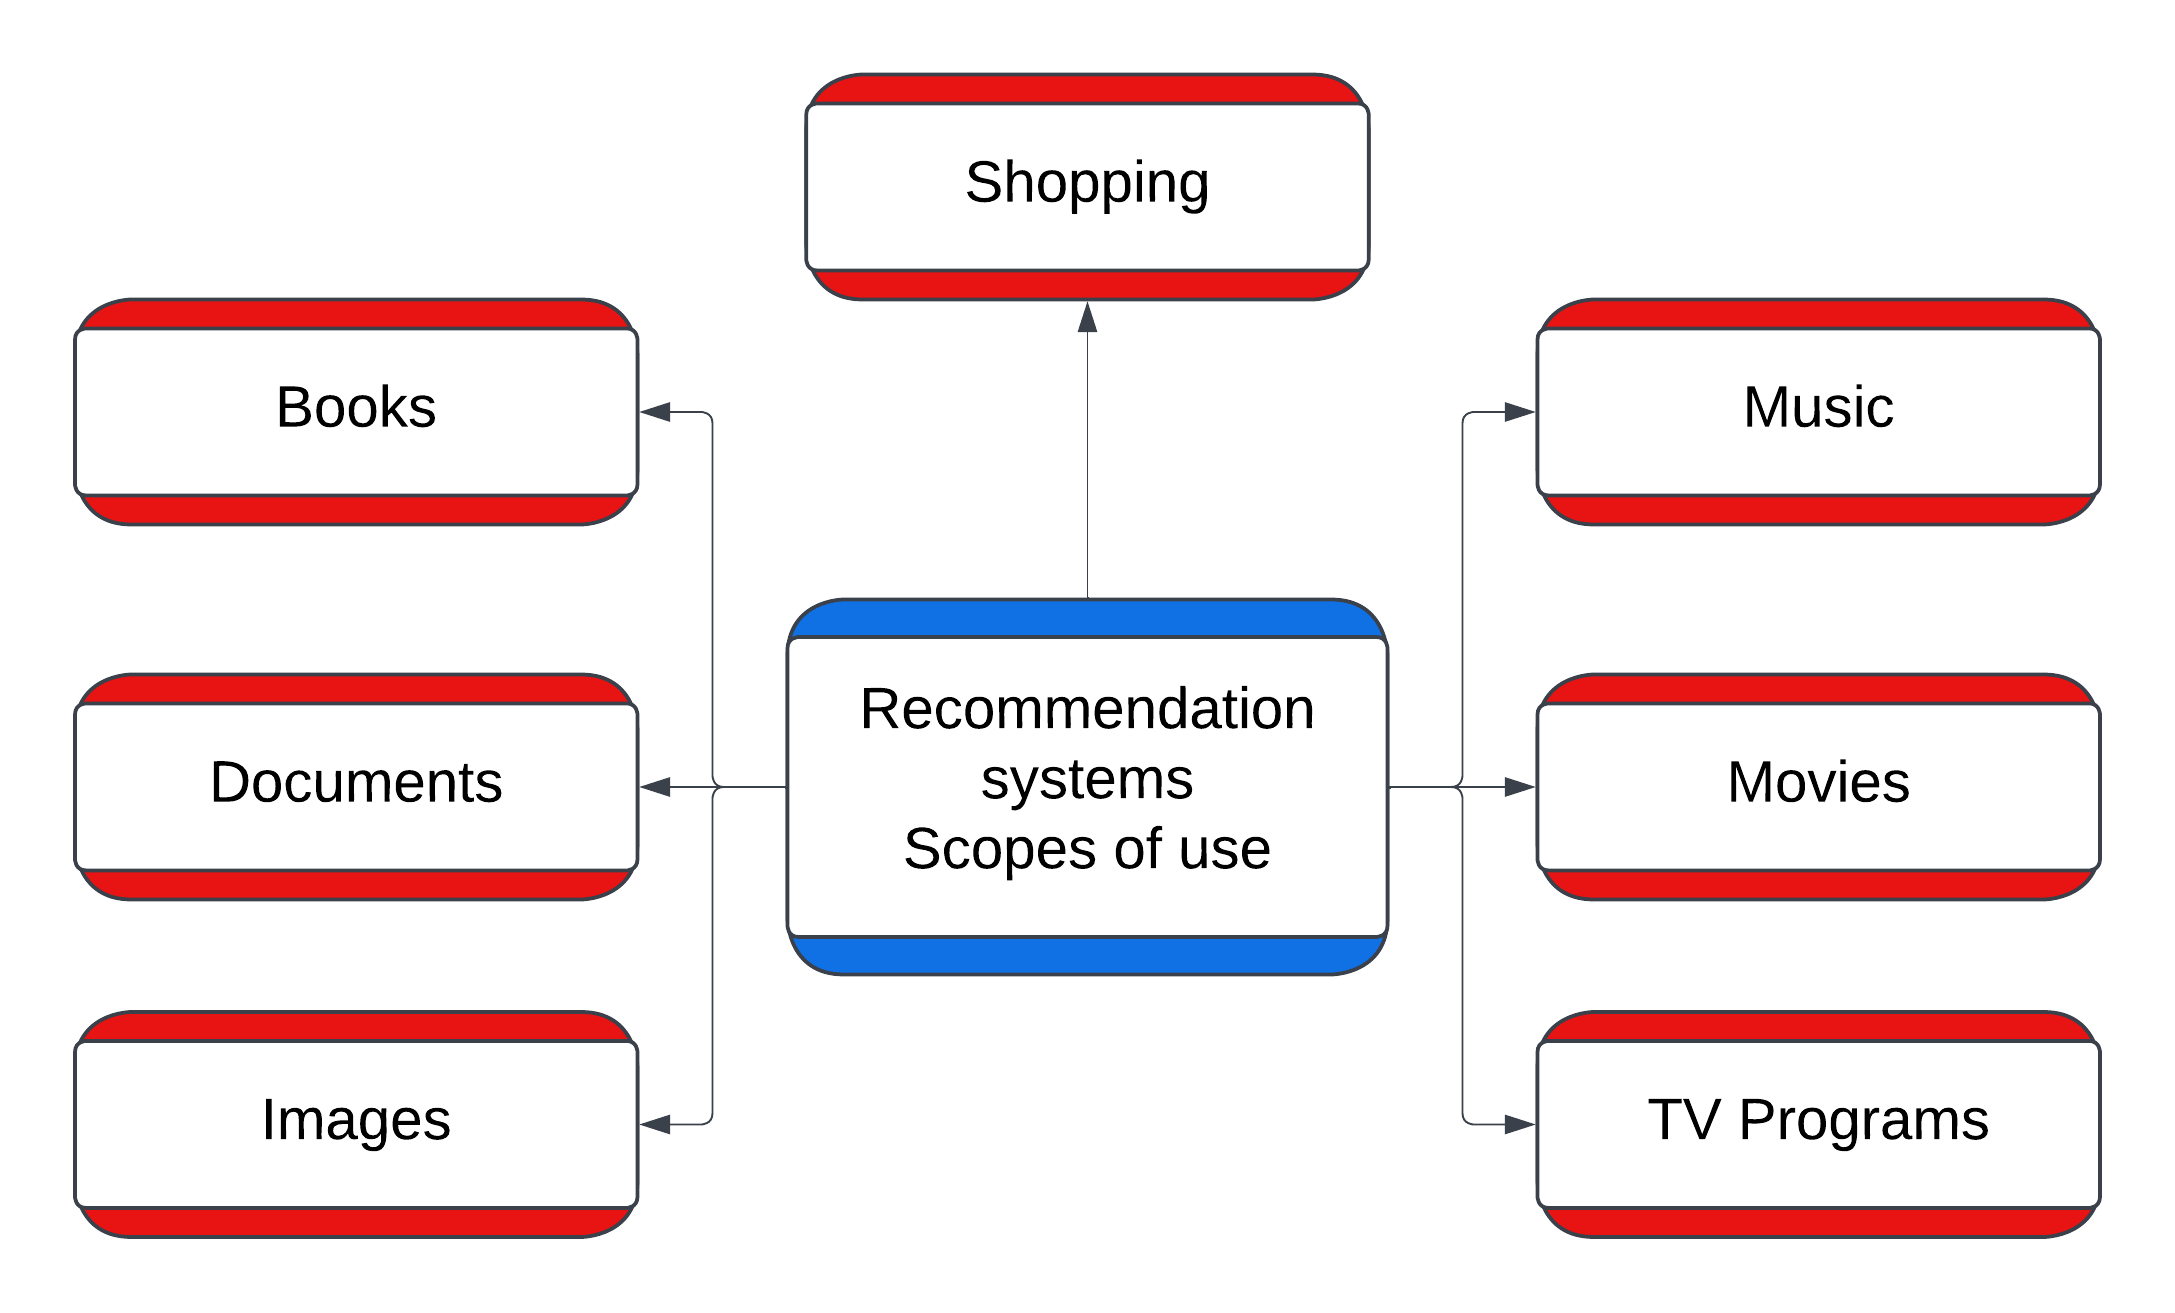
\includegraphics[width=0.8\textwidth]{system_types}
\caption{Most commonly used system types}
\label{fig:Types}
\end{figure}
\newpage










\section{Architecture and principles of workflow}
\subsection{Architecture}
Blah blah blah...

\begin{figure}[h]
\centering
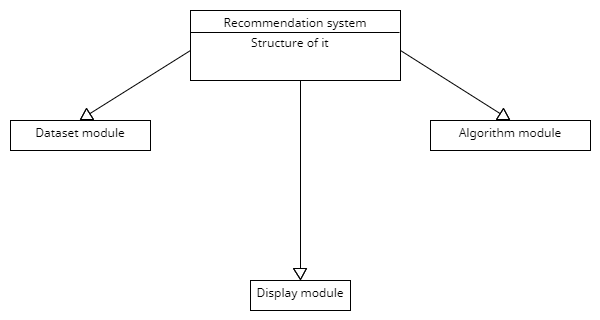
\includegraphics[width=0.8\textwidth]{system_structure}
\caption{Structure of most systems}
\label{fig:Types}
\end{figure}



Some of the \textbf{greatest} discoveries in \underline{science}  were made by \textbf{\textit{accident}}.




\bibliography{literature}
\bibliographystyle{plain}

%Shcolar - https://link.springer.com/chapter/10.1007/978-981-13-7025-0_34
%Scolar - https://www.sciencedirect.com/science/article/pii/S0957417412002825#f0005 
\end{document}
